\begin{figure}[h]
\begin{center}
\bgroup 
 \def\arraystretch{0.2} 
 \setlength\tabcolsep{0.2pt}
\begin{tabular}{cccc}
 & Classification & Ours & \\
 L2 \cite{zhang2016colorful} & (rebal.) \cite{zhang2016colorful} & (L1 + cGAN) & Ground truth \\
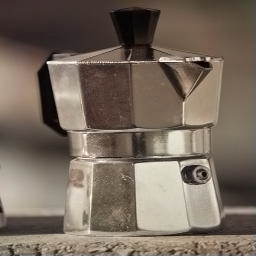
\includegraphics[width=0.25\linewidth]{figs/colorization_colorization_latex/L2_zhang2016_33094.png} &
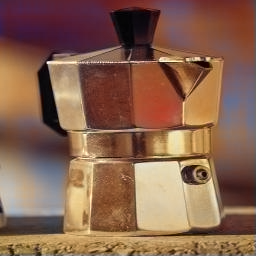
\includegraphics[width=0.25\linewidth]{figs/colorization_colorization_latex/classrebal_zhang2016_33094.png} &
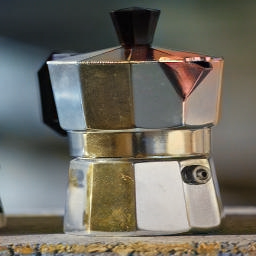
\includegraphics[width=0.25\linewidth]{figs/colorization_colorization_latex/L1cGAN_33094.png} &
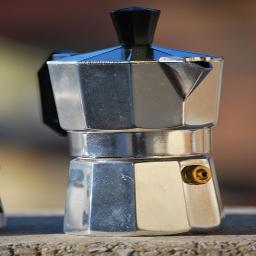
\includegraphics[width=0.25\linewidth]{figs/colorization_colorization_latex/gt_33094.png} \\ 
% \includegraphics[width=0.25\linewidth]{figs/colorization_colorization_latex/L2_zhang2016_42366.png} &
% \includegraphics[width=0.25\linewidth]{figs/colorization_colorization_latex/classrebal_zhang2016_42366.png} &
% \includegraphics[width=0.25\linewidth]{figs/colorization_colorization_latex/L1cGAN_42366.png} &
% \includegraphics[width=0.25\linewidth]{figs/colorization_colorization_latex/gt_42366.png} \\ 
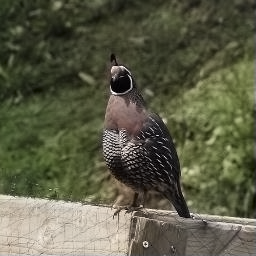
\includegraphics[width=0.25\linewidth]{figs/colorization_colorization_latex/L2_zhang2016_43989.png} &
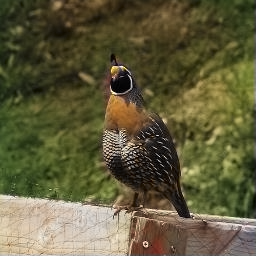
\includegraphics[width=0.25\linewidth]{figs/colorization_colorization_latex/classrebal_zhang2016_43989.png} &
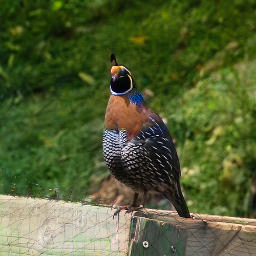
\includegraphics[width=0.25\linewidth]{figs/colorization_colorization_latex/L1cGAN_43989.png} &
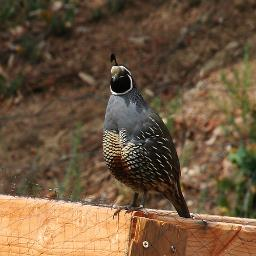
\includegraphics[width=0.25\linewidth]{figs/colorization_colorization_latex/gt_43989.png} \\ 
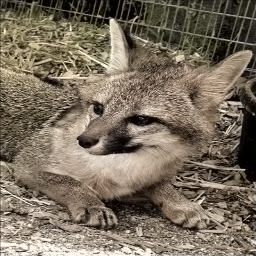
\includegraphics[width=0.25\linewidth]{figs/colorization_colorization_latex/L2_zhang2016_44956.png} &
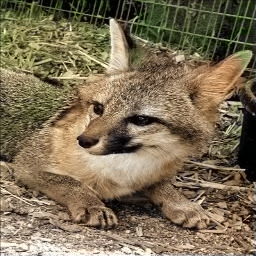
\includegraphics[width=0.25\linewidth]{figs/colorization_colorization_latex/classrebal_zhang2016_44956.png} &
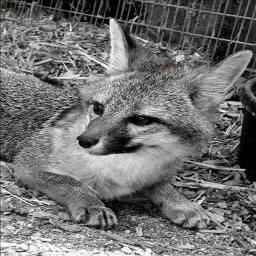
\includegraphics[width=0.25\linewidth]{figs/colorization_colorization_latex/L1cGAN_44956.png} &
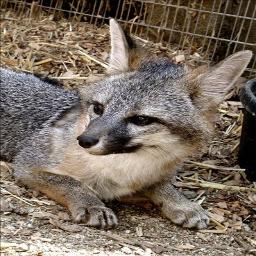
\includegraphics[width=0.25\linewidth]{figs/colorization_colorization_latex/gt_44956.png} %\\ 
%\includegraphics[width=0.25\linewidth]{figs/colorization_colorization_latex/L2_zhang2016_45617.png} &
%\includegraphics[width=0.25\linewidth]{figs/colorization_colorization_latex/classrebal_zhang2016_45617.png} &
%\includegraphics[width=0.25\linewidth]{figs/colorization_colorization_latex/L1cGAN_45617.png} &
%\includegraphics[width=0.25\linewidth]{figs/colorization_colorization_latex/gt_45617.png}

\end{tabular} \egroup 
\end{center}
\vspace{-0.1in}
\caption{Colorization results of conditional GANs versus the L2 regression from \cite{zhang2016colorful} and the full method (classification with rebalancing) from \cite{zhou2016learning}. The cGANs can produce compelling colorizations (first two rows), but have a common failure mode of producing a grayscale or desaturated result (last row).}
\vspace{-0.1in}
\label{colorization_res}
\end{figure}